%(CHECK Version/Carlo 21.11)\\
In diesem Kapitel werden Werkzeuge vorgestellt, mit denen Budgets mit Alarmen erstellt werden, diese informieren die Nutzer, wenn ein bestimmter Prozentsatz des festgelegten Budgets überschritten wurde. Die Erstellung von Budgets trägt zu einer besseren Planung-/Prognose- und Kostenkontrolle. [WEIL, Cost Controlling]
Die Einstellung von Alarmen für relevante Ereignisse wie im Fall einer Budgetüberschreitung oder dem Start einer Instanz[IST GUT WEIL/TRÄG ZU...BEI].

Darüber hinaus ist es mit Werkzeugen wie CloudWatch möglich, die Abschaltung bestimmter Dienste zu automatisieren, wenn eine Budgetschwelle überschritten wurde. Diese Maßnahmen werden in dem nächsten Kapitel genauer behandelt.
[TRUSTED ADVISOR fehlt noch in der Einleitung]
[SOLLTE AB HIER EINE NEUE UNTERKAPITEL ANFANGEN? zb. TAGS ZUR TRENNUNG DER Ressourcen]
Durch die Verwendung von Tags ist es möglich, die Ressourcen nach Kriterien wie Region, Umgebung, Projekt, Art der Ressource usw. zu visualisieren, dies %es
ermöglicht, Kosten auf den von der Organisation festgelegten Ebenen zu verfolgen.

\begin{figure}[h!]
  \centering
  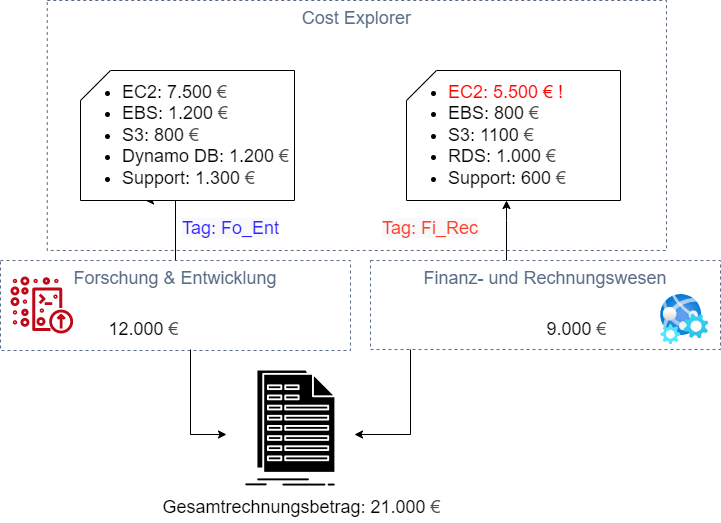
\includegraphics[scale=0.4]{sources/Kosten_Ueber_Abteilungen}
  \caption[Trennung der Kosten durch Tags]{}
  \label{fig:Kosten_Ueber_Abteilungen} 
  Trennung der Kosten durch Tags.\\
  Die Angaben dienen nur als Beispiel und entsprechen keiner realen IT-Infrastruktur.
  %\cite{AMZ20}
\end{figure}

Es könnte zum Beispiel ein Szenario entstehen, in dem eine Abteilung innerhalb einer Organisation mehr Kosten verursacht als Andere. Dies ist nur durch den Anstieg der von Amazon generierten Rechnung, aber um den Grund für diesen Anstieg genauer zu verstehen, muss ihre Ursache untersucht werden. Werkzeuge wie Cost-Explorer machen diese Art von Analyse möglich.

%Zu diesem Zweck werden Werkzeuge vorgestellt, die die Überwachung aktiver Ressourcen ermöglichen.
%Welche Kosten sind mit der Nutzung dieser Werkzeuge verbunden?
%Es sollte gezeigt werden, die Arten/Kategorien von Kunden, die kostenlosen Zugang zu diesen Werkzeuge haben?
%WAS MIT AWS Budgets? AWS Bill and cost Man.?

\subsection{AWS CloudWatch}
%https://aws.amazon.com/de/cloudwatch/pricing/
%https://docs.aws.amazon.com/AmazonCloudWatch/latest/monitoring/GettingStarted.html
Amazon CloudWatch ermöglicht die Überwachung der Leistung von Resources, auch bei Ressourcen, die über verschiedene Regionen verteilt sind. CloudWatch sammelt operative Daten für die Verlaufsanalysen und die Entscheidungsfindung in Bezug auf Optimierung und Fehlerbehebung. CloudWatch beschränkt sich nicht nur darauf, Daten aus der AWS-Umgebung zu empfangen. Externe Metriken, die mit CloudWatch kompatibel sind, können für eine einheitliche Analyse aggregiert werden. Eine der Metriken, die mit Amazon CloudWatch überwacht werden kann, ist die CPU-Auslastung von EC2-Instanzen. Basierend auf einem Prozentsatz der CPU-Auslastung können Benachrichtigungen und Aktionen konfiguriert werden. Eine dieser Aktionen ist die automatische Einrichtung neuer Instanzen zur Deckung des Kapazitätsbedarfs\footnote{\cite{AWS1},AWS Certified Solutions Architect - Associate (SAA-C02), Seite 185}. Diese Art von Aktionen werden im Kapitel ~\ref{kap_Optimierung} tiefer behandelt.
\\\\
Im Folgenden werden die grundlegenden Bereiche und Begriffe von CloudWatch erläutert und wie sie zur Überwachung von Informationen über AWS-Ressourcen verwendet werden.
\\\\
\textbf{Metriken} \\
Eine Metrik stellt eine Reihe von Daten über die Leistung einer Ressource in zeitlicher Reihenfolge dar. Standardmäßig werden viele kostenlose Metriken an CloudWatch übermittelt.
\begin{comment}\\
Metriken bleiben wie folgt verfügbar:\\
Auflösung/Zeitraum: \\
1 Minute - 15 Tage\\
5 Minuten - 63 Tage.\\
1 Stunde - 15 Monate
\footnote{\cite{AMZ15}, Wie lange werden die verfügbaren Metriken aufbewahrt?}
\end{comment}
Zum Beispiel kann der Durchschnitt von einer bestimmten API pro Stunde untersucht werden.
Für eine detailliertere Überwachung ist es möglich, benutzerdefinierte Metriken zu konfigurieren, die eine Auflösung von bis zu eine Sekunde zulassen. Ein praktisches Beispiel für benutzerdefinierte Metriken ist die Messung der Ladezeit einer Website.
[ANDERES BEISPIEL?]
% MIT BEZUG AUF K:OPTIMIERUNG?oder WIESO IST DIE AUFLÖSUNG RELEVANT?]
%\textbf{Logs} \\ BRAUCHE ICH DAS?
\\\\
\textbf{Ereignisse} 
\\
Bei CloudWatch wird eine Änderung bei einer Ressource in der AWS-Umgebung Ereignis genannt. 
AWS-Ressourcen können Ereignisse erzeugen, wenn sich ihr Status ändert.
Beispielsweise, wird ein Ereignis erzeugt, wenn Amazon EC2 Auto Scaling, Instanzen gestartet oder beendet werden\footnote{\cite{AMZ13}, AWS Cloud Watch Events: User GuideSeite 1} oder wenn eine bestimmte Menge an Speicherplatz in einem Bucket erreicht wurde. Ein Bucket ist ein Behälter, in dem Objekte bei Amazon S3 gespeichert werden\footnote{\cite{AMZ18}Amazon Simple Storage Service User Guide, Seite 4}. Beispiele für Objekte sind Dateien wie Bilder und Videos. 
\\\\
\textbf{Regel} \\
Eine Regel ordnet eintreffende Ereignisse zu und leitet diese zur Verarbeitung an Ziele weiter.
Eine einzelne Regel kann an mehrere Ziele weiterleiten, die alle parallel verarbeitet werden\footnote{\cite{AMZ13}, AWS Cloud Watch : User Guide, Seite 2}.
\\\\
\textbf{Ziele} \\
Ziele oder Targets sind Ressourcen, die aufgerufen werden, wenn eine Regel ausgelöst wird.
EC2 instances, AWS Lambda functions und Amazon SNS sind unter anderem mögliche Ziele.
Die Ziele einer Regel müssen sich in derselben Region wie die Regel befinden
\footnote{\cite{AMZ13}, Seite 2}.
%Alle zugelassene Ressourcen \footnote\url{https://docs.aws.amazon.com/AmazonCloudWatch/latest/events/EventTypes.html}
\\\\
\textbf{Benachrichtigungen}\\
%https://docs.aws.amazon.com/AmazonCloudWatch/latest/monitoring/AlarmThatSendsEmail.html
Benachrichtigt zu werden ist wichtig, um relevante Ereignisse nicht zu verpassen und rechtzeitig Maßnahmen zu ergreifen. Mit CloudWatch können Alarme eingerichtet werden, die durch Metriken wie die CPU-Auslastung und auch Gebühren[PASSENDES WORT?] auf AWS-Rechnungen ausgelöst werden.
Benachrichtigungen können durch Amazon SNS\footnote{Amazon SNS ist ein Dienst, der die Benachrichtigung an Personen und an Applikationen ermöglicht. https://aws.amazon.com/de/sns/} oder zu einer E-Mail-Adresse geschickt werden.
%AUCH PER SLACK ODER ÄHNLICHES
\\\\
%This could be a good example %https://youtu.be/__knpcBRLHg?t=770
%https://docs.aws.amazon.com/autoscaling/ec2/userguide/Cooldown.html
%Autoscaling group seted with cooldown periods to avoid too much instances to by launched.
%Most popular parts of CloudWatch:
%https://youtu.be/k7wuIrHU4UY?t=785
% LINKS :
%https://docs.aws.amazon.com/AmazonCloudWatch/latest/monitoring/GettingStarted.html
%https://docs.aws.amazon.com/AmazonCloudWatch/latest/monitoring/WhatIsCloudWatch.html
%https://docs.aws.amazon.com/AmazonCloudWatch/latest/monitoring/Install-CloudWatch-Agent.html
\textbf{Visualisierung von Metriken}\\
Mit Cloud-Watch Dashboards können relevante Metriken grafisch dargestellt werden. %[BESSERE FORMULIERUNG] %Sie ermöglichen eine umfassende Visualisierung von Metriken der Ressourcen in der AWS-Umgebung. 
Durch die Dashboards können auch Benachrichtigungen erstellt werden. Für die Einrichtung der Benachrichtigungen ist kein technisches Wissen nötig\footnote{\cite{AMZ14},AWS Cloud Watch : User Guide, Seite 28}.
%Die von CloudWatch gesammelte Informationen sind nicht nur für System-Administratoren relevant.
Die in den Dashboards enthaltenen Informationen sind nicht nur für ihre Autoren von Relevanz.
Weitere Personen innerhalb oder außerhalb der Organisation können Zugriff auf Dashboards mit nützlichen Informationen bekommen, um Prozesse zu beschleunigen[VORTEILE DES OPTIMIERUNGSPROZESS VERWEISEN] oder Probleme schneller zu beheben[USE CASE].

Dies ermöglicht einen schnelleren Kommunikationsfluss in Echtzeit[Fach Informationsmanagement: (Schwachstellenanalyse) IuM Technik/Check Book KCrmar]. Die Zugriffsverwaltung für geteilte Dashboards wird über AWS Identity and Access Management abgewickelt\footnote{\cite{AMZ14}, Seite 18 und 39}[UND?].
\\\\
\subsubsection*{Fakturierungsalarme mit CloudWatch}
%Seite 145 Amazon CloudWatch - Benutzerhandbuch
AWS CloudWatch empfängt Abrechnungsmetriken von alle Ressourcen. Auf der Grundlage dieser Metriken ist es daher möglich, Regeln zu erstellen, die bei Überschreitung des geplanten Budgets einen Alarm auslösen.
%[KANN MAN NUR Total Estimated Charge verwenden ODER KÖNNTE MAN NACH PROJEKTE TRENNEN?]
[BEZUG AUF PROJEKTMANAGEMENT/Kostenkontrolle?]

\subsubsection*{Benachrichtigung bei Hoch- und Runterfahren von EC2-Instanzen}
Obwohl Auto-Scaling dafür sorgt, die Rechenkapazität dynamisch anzupassen, ist es von größter Wichtigkeit, über Änderungen in der Infrastruktur informiert zu sein, ohne die Dashboards manuell überprüfen zu müssen.
[WEIL ....]
\\\\
\subsection{AWS Cost-Explorer}
Mit Cost-Explorer können Kosten der letzten 12 Monate und eine Schätzung der Kosten des laufenden Monats visualisiert werden. Darüber hinaus wird eine Kostenprognose für die nächsten Monate erstellt. Die Prognose basieren auf die Kosten der vergangenen Monaten. Die Nutzung des Cost-Explorers ist kostenlos, nur API-Aufrufe sind kostenpflichtig \footnote{{\cite{AMZ22}AWS Cost Management Pricing}}.
\\
%Mio:%Conocer clos costos en un periodo de tiempo nos permite %saber si estamos en el camino correcto para alcanzar las %metas trazadas al inicio del periodo/proyecto y tomar %las medidas adecuadas para que al final del periodo/%proyecto tengamos resultados satisfactorios.
Amazon analysiert die bisherige Nutzung der Instanzen und gibt Empfehlungen zur Kostensenkung durch den Wechsel von EC2-Instanzen in On-Demand Zahlungsmodell zu reservierten Instanzen. Diese ignorieren Kapazität, die bereits von anderen reservierten Instanzen abgedeckt wurden.
Es besteht die Möglichkeit, einen Bericht über die Ressourcennutzung der letzten 12 Monate einzusehen und zu prüfen, ob die Empfehlungen des Cost-Explorers angemessen sind.

\subsubsection*{Budgetplanung}
Die Budgetplanung ist eine Methode der Kostenkontrolle, die beim Start eines neuen Projekts eingesetzt wird\footnote{\cite{BUD2}Cost Control Methods: Definitions and Examples}. Der Bericht über die in den letzten 12 Monaten entstandenen Kosten zusammen mit der Prognose der Kosten der kommenden drei Monaten tragen zu einen guten Budgetplanung bei.
%%t.ly/6bvZ% https://youtu.be/3peNAKB3VxA?t=223
Durch die Möglichkeit, die in den letzten Monaten angefallenen Kosten nach Ressourcen, Projekt oder Abteilung zu trennen, ist es möglich, operative Budgetplanungen aus vergangenen Projekten mit Genauigkeit zu erstellen. 
\begin{quote}
  „Bei der operativen Planung wird von einem Zeithorizont von einem Jahr ausgegangen. Hier liegt der Fokus darauf, Ressourcen konkret zuzuweisen und detailreicher zu planen. Welche Mittel werden wofür verwendet und welche kurz- und mittelfristigen Ziele sollen durch diesen Mitteleinsatz erreicht werden”\cite{BUD1}.
\end{quote}

Cost-Explorer liefert Informationen zur Rechtfertigung von Ausgaben aus im Voraus festgelegten Budgets, hilft bei der Planung künftiger Budgets und unterstützt die []
%\textbf{Aktuelle Budgets vs erwartet=Soll-Ist-Vergleich Methode}
%Einer der Standardberichte im AWS Cost Explorer enthält die Kosten in Dollar/Euro und die Nutzung von EC2-Instanzen in Stunden pro Monat. Mit diesen Informationen können Sie die Kosten für eine bestimmte Dienstleistung berechnen. 
\subsection{AWS Trusted Advisor}
%https://www.youtube.com/watch?v=i0IkKN9NoPk
%https://aws.amazon.com/de/premiumsupport/technology/trusted-advisor/
%Kunden von AWS Basic Support und AWS Developer Support können auf grundlegende Sicherheitsprüfungen und alle Prüfungen für Servicekontingente zugreifen. Kunden von AWS Business Support und AWS Enterprise Support können auf alle Prüfungen zugreifen, einschließlich Kostenoptimierung, Sicherheit, Fehlertoleranz, Leistung und Servicekontingente. 
%was macht dieses?
%AWS Trusted Advisor: This helps you know more about idle or underutilized resources.

AWS Trusted Advisor ist ein Werkzeug, das entwickelt wurde, um Kosten zu senken, um Systemverfügbarkeit und -leistung zu verbessern und um Sicherheit zu erhöhen. Es analysiert die Nutzung des AWS-Kontos und gibt Best-Practice-Empfehlungen. Es werden die Kategorien Leistungsgrenzen und Kostenoptimierung insbesondere betrachtet, da diese am relevanten für die vorliegende Arbeit sind. Es ist zu berücksichtigen, dass nur limitierte Sicherheitsprüfungen (6 Prüfungen November 2021) für Konten in den Plänen Developer und Basic Support kostenlos sind. Prüfungen für die Kategorie Leistungsgrenzen sind kostenlos. Detaillierte Informationen und Empfehlungen von der Kategorien Kostenoptimierung, Performance und Fehlertoleranz sind nur zugänglich, wenn ein Business- oder Enterprise-Konto vorliegt\footnote{https://aws.amazon.com/de/premiumsupport/technology/trusted-advisor/}. \\
%ES MUSS GEPRÜFT WERDEN, OB ES SINNVOLL IST, FÜR DIE OBEN GENANNTEN SUPPORT-PLÄNEN ZU ZAHLEN.

\begin{figure}[h!]
      \centering
      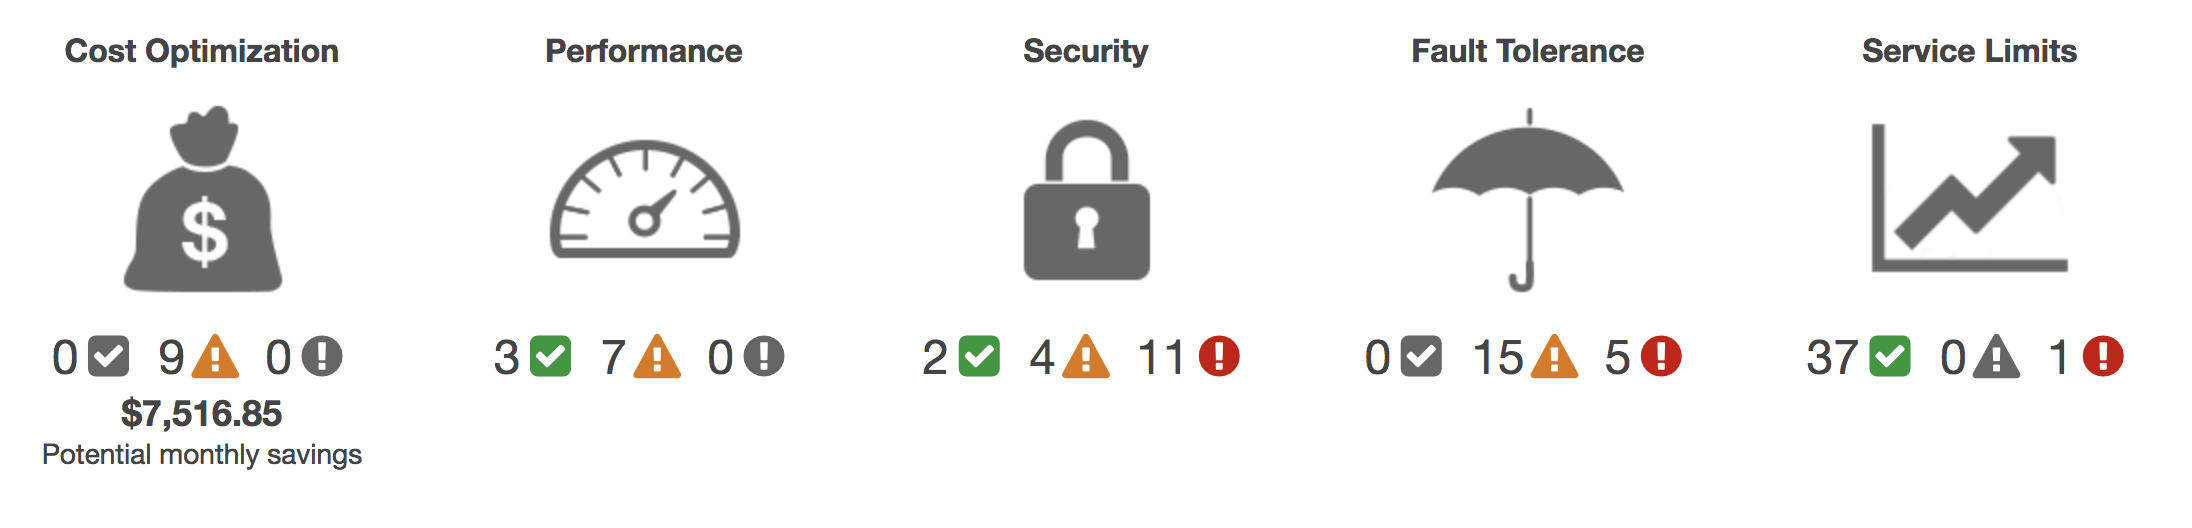
\includegraphics[scale=0.4]{sources/AWS_Trusted_Advisor_Kategorien}
      \caption[AWS Trusted Advisor Kategorien]{}
      \label{fig:AWS_Trusted_Advisor_Kategorien} 
      AWS Trusted Advisor Kategorien\cite{AMZ20}
\end{figure}
Die \autoref{fig:AWS_Trusted_Advisor_Kategorien} zeigt die fünf Kategorien von Trusted Advisor mit jeweils 3 Arten von Indikatoren. Die Indikatoren zeigen an, welche Prüfungen durchgeführt wurden. Grün bedeutet, dass keine Fehler oder zu prüfenden Empfehlungen vorhanden sind. Warnungen werden durch orangefarbene Indikatoren und Fehler durch rote Indikatoren angezeigt. Diese Empfehlungen sind eine Zusammenfassung auf hohem Niveau. Sie sind ein Startpunkt für die Untersuchung von Ressourcen mit Hilfe anderer Werkzeuge wie CloudWatch oder Cost-Explorer.%[ODER?].
\\\\

\subsubsection*{Kostenoptimierung}
Die Empfehlungen zur Kostenoptimierung konzentrieren sich auf Möglichkeiten zur Kostensenkung, indem ungenutzte Ressourcen hervorgehoben werden. 
Sollten EC2-Instanzen mit geringer Auslastung gefunden werden, wird es diese bei Trusted Advisor signalisiert. Denn diese Instanzen verbrauchen Ressourcen und können terminiert oder pausiert werden. %[HIER FEHLT...]
Auch nicht zugewiesene Elastic IP-Adressen erzeugen Kosten. Diese können gegebenenfalls von Trusted Advisor gefunden werden. %t.ly/nYiv
[BEISPIELE]

\subsubsection*{Leistungsgrenzen}
In dieser Kategorie werden Empfehlungen zur Vermeidung von Grenzwertüberschreitungen hervorgehoben.
Es wird zum Beispiel nach einer Nutzung gesucht, die mehr als 80 \% des Leistungsgrenzwerten für wichtige Dienste beträgt. Einige Beispiele sind  Amazon EC2, Auto Scaling, Elastic Block Store, Simple Email Service und AWS CloudFormation.
\\\\
Sich dieser Grenzen bewusst zu sein, gibt die Möglichkeit, rechtzeitig zu handeln und es trägt zu Kostenüberwachung bei.
[GLEICHE GRENZEN WIE BEI CloudWatch?]
Bei der Erwägung von Trusted-Advisor ist zu überlegen, ob es kosteneffizient ist, für Pläne zu zahlen, die den Zugang zu allen Empfehlungen des Trusted Advisors ermöglichen. Das übergeordnete Ziel dieser Arbeit ist es, die Entstehung der Kosten auf eine praktikable Weise zu verstehen (Kostenüberwachung). Dies, um Optimierungsmaßnahmen zu ermöglichen. 
\\
Es wäre nicht sinnvoll, Kosten für Plänen wie Geschäfts- oder Enterprise Support zu übernehmen, wenn diese die möglichen Einsparungen übersteigen.  Die Vorteile von Geschäfts- oder Enterprise Support-Plänen beschränken sich nicht auf Kosteneinsparungen und Kostenbegrenzung, sondern tragen auch zur Sicherheit und Leistung bei. Jedes Unternehmen muss selbst entscheiden, ob es diese Informationen benötigt.
[ZEIGE BEISPIELE FueR Empfehlungen]\\
%[WIE TRIFFT MAN EINE ENTSCHEIDUNG IM UNTERNEHMEN? MODELLE?]
\\
\subsection{Überwachungswerkzeuge gemäß ihrer Verwendung}
Die \autoref{fig:ÜberwachungswerkzeugeNachVerwendung} fasst die Überwachungswerkzeuge zusammen und listet die Verwendung der einzelnen Werkzeuge auf.
\begin{figure}[h!]
  \centering
  \includegraphics[scale=0.6]{sources/ÜberwachungswerkzeugeNachVerwendung}
  \caption[Überwachungswerkzeuge gemäß ihrer Verwendung]{}
  \label{fig:ÜberwachungswerkzeugeNachVerwendung} 
  Überwachungswerkzeuge gemäß ihrer Verwendung\\
  Eigene Darstellung\cite{AMZ12, AMZ20, AMZ21}. 
\end{figure}
[NOCH NICHT VOLLSTÄNDIG]

\subsection*{Handlungsempfehlungen}
[SIND SIE HIER RICHTIG PLAZIERT? SOLLTEN LIEBER IN FAZIT SEIN?;NOCH ZU VERVOLSTÄNDIGEN]
\\\\
\subsection*{Handlungsempfehlung 1:} 
Es kann in Erwägung gezogen werden, für einen begrenzten Zeitraum von 3 Monaten einen Support-Plan zu bezahlen, um aus den gegebenen Empfehlungen zu lernen. Oder Business-Plan alle 6 Monate für 1 Monat zu aktivieren.  
\\\\
\subsection*{Handlungsempfehlung 2:} 
Ein Berater für eine Prüfung und Optimierung der Ressourcen kann in Deutschland zwischen x und N-EUR kosten. Dies ist eine Alternative zu den Plänen des Trusted-Advisor. Ein Berater, der alle 5 Kategorien abdeckt, könnte [BETRAG] kosten. %Das sagt der Berater Juanito von der Firma XXX.
\\\\
\subsection*{Fazit}
%[ABSCHLUSS DES KAPITELS/Überbrückung FÜR DAS KOMMENDE KAPITEL]}
% CloudWatch
In diesem Kapitel wurde gezeigt, dass es mit CloudWatch möglich ist, Alarme auf Basis von Ereignissen einzurichten, die mit Amazon SNS oder externen E-Mail-Adressen kommunizieren. Im nächsten Kapitel wird CloudWatch erneut behandelt. Diesmal nicht als Überwachungswerkzeug, sondern als Optimierungswerkzeug zur Erstellung von automatisierte Aktionen/Reaktionen. Dazu war es notwendig, die Rolle der von CloudWatch gesammelten Metriken zu verstehen, die die Grundlage für die Verwaltung von Aktionen wie Auto-Scaling-Gruppen bilden. 
%Cost Explorer
Aus dem Blickwinkel des Kostenmanagements wurde gezeigt, dass mit Cost-Explorer eine Analyse von Kosten der letzten 12 Monate, eine Einschätzung der Kosten im aktuellen Monat und eine Prognose für die nächsten Monate möglich ist. Diese Informationen dient unter anderem zur Erstellung einer operativen Budgetplanung mit genaueren Daten, da
Kosten nach Tags und anderen Filtern getrennt werden können.
%Trusted Advisor
Darüber hinaus wurde Trusted Advisor vorgestellt, die konkrete Optimierungsempfehlungen gibt und warnt über Leistungsgrenzen. Dies kann mit erheblichen Kosten verbunden sein und ist daher nicht für alle Arten von Unternehmen unmittelbar attraktiv. Obwohl sich nicht alle Unternehmen die Prüfungen von Trusted Advisor leisten können, sollten die kostenlosen Empfehlungen im Überwachungs- und Optimierungsplan berücksichtigt werden.
[WAS KOMMT IN NÄCHTEN KAP.?]

\begin{comment}
En este capitulo se  mostró de qué manera es posible con CloudWatch configurar alarmas basadas en eventos. Dichas alarmas comunican con Amazon SNS o direcciones de correo externas. En el capiulo siguiente se volverá a tematizar CloudWatch. Esta vez no como herramienta de monitoneo, sino de optimizacion para crear acciones ??? Para ello fue necesario entender que papel juegan las metricas recolectadas por CloudWatch, las cuales son la base para manejar los grupos Auto-Scaling. 

Desde la perspectiva del manejo de costos, se mostró como con Cost-Explorer es posible analizar los costos de los ultimos 12 meses, tener un calculo de los costos en el mes actual y recibir un pronostico de los proximos meses. Teniendo la posibilidad de separar los costos por medio de Tags y otros filtros. Dicha información contribuye a poder crear una planificacion de presupuestos operativa basada en datos de gran presicion.

Además se presentaron herramientas como Trusted Advisor las cuales brindan recomendaciones concretas sobre optimizacion y alertan si limites que se acercan a su umbral máximo. 

Este puede representar costos consideradable y que por lo tanto no lo hacen directamente atractivo para todo tipo de empresas.
\end{comment}

\begin{comment}
AWS Cost-Explorer Budgets show actual spend vs budget by month.
Filter by budgets, tags and tax, region, instances, usage type, cost category
Die Kosten vorhersehbar machen
Wiederverwendung gespeicherter Berichte. Welche Vorteile?

Da kann man sehen wie viele Stunden an RI und an On-Demand pro Tag/Monat verbraucht wurden.
-	Informationen um Schätzungen handelt, die von den tatsächlichen Kosten für den Abrechnungszeitraum abweichen können. %https://youtu.be/3peNAKB3VxA?t=705
-	Kann ich die Usage von S3 Einheiten und analysieren, wie häufig diese zugegriffen werden %https://youtu.be/pjrKDkzbas8?t=2425
-	Man könnte herausfinden, ob die RIs tatsächlich günstiger als ON-Demand sind. Wenn die RIs sind „konvertierbar“ und teurer als On-Demand, könnte man sich dafür entscheiden diese in was umzuwandeln, was genutzt wird. %https://youtu.be/pjrKDkzbas8?t=3385

%(How to use Spots and on-demand)
%detect CPU Utilization, with Amazon CloudWatch
\end{comment}
%IST taging EINE STRATEGIE?
%I could compute the cost of a query, user, transaction
% https://youtu.be/qYHR_V1lvNU?t=375